 %!TEX root = ../thesis.tex
%*******************************************************************************
%*********************************** Introduccion *****************************
%*******************************************************************************

\chapter{Introducción}\label{chap:intro}

La interacción de los factores naturales y antrópicos es el origen de la estructura espacial compleja y heterogénea que presenta el paisaje \citep{Forman1986,Turner2001}. En las últimas décadas, la ecología del paisaje ha estudiado la configuración, el tamaño y la forma de los componentes que estructuran el territorio utilizando \textbf{métricas de paisaje} \citep{Aguilera2010}. Hoy en día, para estudiar la estructura del paisaje se dispone de \textbf{gran cantidad de información y herramientas}. 

Las bases de datos de ocupación del suelo, como por ejemplo el Sistema de Información de Ocupación del Suelo en España (SIOSE), representan el territorio de un modo adecuado para aplicar conceptos fundamentales como los de conectividad o diversidad del paisaje. Además, estas bases de datos aumentan progresivamente en riqueza semántica y resolución geométrica, por lo que \textbf{la información disponible no para de crecer}.

Complementariamente, también existe software específico o de carácter más general que facilita el cálculo de métricas del paisaje. Sin embargo, \textbf{ninguna de las aplicaciones encontradas es lo suficientemente escalable y extensible como para analizar grandes bases de datos de ocupación del suelo tan complejas como las actuales} (p.ej. SIOSE). 

Evidentemente, los problemas existentes al analizar las geodatabases actuales irá en aumento con la cada vez mayor disponibilidad de datos obtenidos a partir de imágenes de satélite o datos de campo. Este trabajo se enmarca en este contexto de creciente complejidad y busca \textbf{proponer herramientas más sencillas y eficientes en el cálculo de métricas del paisaje}.


\section{El SIOSE como fuente para el estudio de la estructura del paisaje}\label{sec:siose}

\begin{graybox}
\begin{itemize}
\item El SIOSE es una valiosa \textbf{base de datos de ocupación del suelo} que contiene un gran volumen de información territorial de toda España.
\item Desde su aparición en 2005, SIOSE se ha convertido en un repositorio de referencia para sus homólogos europeos, llegando a ser un \textbf{modelo para la iniciativa EAGLE} (\textit{SIOSE europeo}). 
\item A pesar de su gran potencial, el SIOSE presenta ciertos problemas de \textit{usabilidad} debidos a su gran volumen y complejidad.
\end{itemize}
\end{graybox}


El Sistema de Información de Ocupación del Suelo en España (SIOSE) se lanzó en el año 2005 por la Dirección General del Instituto Geográfico Nacional de España (IGN)\footnote{\url{http://www.ign.es/web/ign/portal}} ante la necesidad de adquirir información más detallada a nivel nacional. El SIOSE está integrado en el Plan Nacional de Observación del Territorio (PNOT) con el objetivo de alcanzar una infraestructura de datos espaciales multidisciplinar. Este conjunto de datos va a ser un componente imprescindible para llevar a cabo los objetivos de este trabajo.

El SIOSE es una base de datos que recoge información de la ocupación del suelo de España en forma de malla continua de polígonos a partir de la fotointerpretación de imágenes. Cada polígono se especifica por dos componentes: la cobertura del suelo (\textit{Land Cover, LC}) se refiere a las características de la cubierta natural, como por ejemplo cuerpos de agua, bosques, superficies urbanas, zonas agrícolas, etc., y el uso del suelo (\textit{Land Use, LU})se define por las funciones socioeconómicas en el territorio, como por ejemplo uso industrial, residencial, forestal, agrícola, etc.

La escala de referencia es 1:25.000 y el sistema geodésico de referencia es European Terrestrial Reference System 1989 (ETRS89) con proyección Universal Transversa de Mercator (UTM). El tamaño mínimo de los polígonos depende del tipo de cobertura: 2 ha para las zonas agrícolas, forestales y naturales, 1 ha para las superficies artificiales y 0,5 ha para agua, cultivos forzados, coberturas húmedas, playas, vegetación de ribera y acantilados. La base de datos del SIOSE ha sido diseñada utilizando un \textbf{modelo orientado a objetos} que describe los objetos, atributos y relaciones de los elementos del territorio. Esto permite la asignación de una o varias coberturas de suelo a un único polígono (datos semiestructurados). Cuando el polígono presente una única cobertura tendrá una \textit{cobertura simple}, pero cuando esté formado por dos o más coberturas tendrá una \textit{cobertura compuesta}, o también conocido como multietiqueta o \textit{multilabel} \citep{EquipoTecnicoNacionalSIOSE2015}. El hecho de que sea un modelo orientado a objetos, garantiza la compatibilidad y comparabilidad con otras bases de datos de ocupación del suelo como por ejemplo el \textit{Corine Land Cover (CLC)}. Sin embargo, físicamente, este modelo se ha descrito como un modelo \textbf{entidad-relación} para poder implementarlo también en bases de datos espaciales relacionales, que son las más utilizadas de hoy en día y las más habituales en los SIG.

\begin{figure}
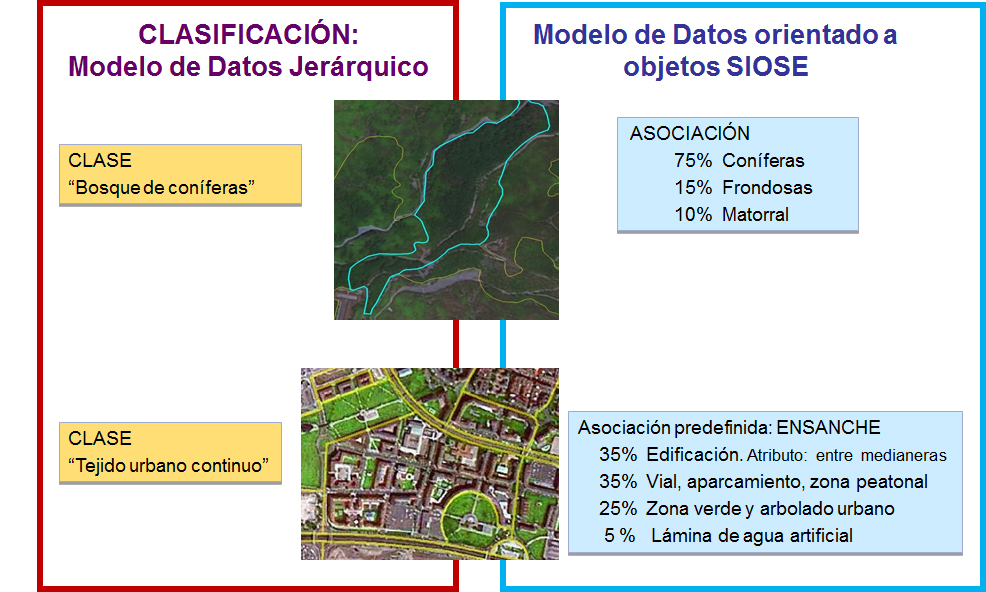
\includegraphics[width=\textwidth]{Introduccion/Figs/siose-oo.png}
\caption{Riqueza descriptiva del modelo de datos orientado a objetos del SIOSE frente a una clasificación jerárquica. Fuente: \url{www.siose.es}.\label{fig:siose-oo}}
\end{figure}

El SIOSE tiene una proyección internacional ya que hay iniciativas similares en otros muchos países. Concretamente, el grupo EAGLE (Eionet Action Group on Land monitoring in Europe) tiene como objetivo solucionar la vigilancia de la tierra sobre la información europea de las fuentes de datos nacionales para una mejor integración y armonización a partir del concepto \textit{bottom-up}, además de facilitar el intercambio y comparación de datos entre países europeos \citep{Arnold2013}. 

El Instituto Geográfico Nacional de España (IGN) creó el SIOSE muy tempranamente (2005) siguiendo los últimos estándares internacionales, por lo que con el tiempo se ha convertido en un repositorio de ocupación del suelo de referencia a nivel europeo \citep{EquipoTecnicoNacionalSIOSE2015}. Del mismo modo, uno de los objetivos futuros del SIOSE es avanzar hacia una base de datos de ocupación del suelo europea para que resulte más fácil trabajar a nivel internacional.

El análisis de la estructura del paisaje a partir de datos de usos y coberturas del suelo ha sido aplicado habitualmente desde diversas disciplinas y ámbitos de estudio. Por ejemplo, se han realizado estudios sobre:

\begin{itemize}
\item Medio Ambiente y hábitats naturales: delimitación de unidades de paisaje \citep{Gine2014}, impacto, abundancia, densidad entre fauna y paisaje \citep{Hamilton2009,Hebeisen2008,Brennan2005}, repercusiones ambientales y transformaciones en el paisaje \citep{GimenezFont2010} y conservación de áreas protegidas para el hábitat de especies \citep{Lin2014}.
\item Demografía, urbanismo y planificación del territorio: análisis de las características de la estructura urbana y perirubana \citep{Aguilera2011,Jacquin2008}, comparación de estructuras \citep{Blaschke1999}, conflictos entre usos de suelo \citep{Tudor2014}, análisis de patrones urbanos \citep{Aguilera2010} y análisis urbano mediante el uso del Atlas Urbano \citep{Prastacos2017}.
\item Infraestructuras, energía y transporte: planificación del uso del suelo y transporte para un corredor de tránsito de tren ligero \citep{Soria-Lara2016}.
\item Dinámica de la ocupación del suelo: reclasificación de usos urbanos \citep{VanderKwast2011}, tipología urbana y conflictos de usos \citep{Dunk2011,Aguilera2012}, uso de la Teledetección para la descripción de estructuras y cambios urbanos \citep{Herold2002}, lagunaridad del paisaje \citep{Roces-Diaz2014}, correlación entre estructuras de categorías y paisaje \citep{Liu2016} y evaluación de la dinámica de usos de suelo \citep{Rodriguez-Rodriguez2017}.
\end{itemize}

También se han realizado estudios sobre abandono agrícola \citep{Zaragozi2011} y otros sobre el riesgo de incendio asociado a nuevas formas de ocupación del suelo \citep{Vazquez2017}.

Los principales usuarios que trabajan con información sobre ocupación del suelo son la Administración General, gobiernos autonómicos, universidades, organismos de investigación, organismos europeos e internacionales, empresas públicas y privadas y, en menor medida, los usuarios particulares. Todos estos usuarios del SIOSE se ven afectados por dos dificultades relacionadas con la \textit{usabilidad} de los datos: \textbf{el gran volumen de datos y la complejidad del modelo de datos}. La base de datos está formada por unos 2,5 millones de geometrías poligonales con sus coberturas de suelo. Este volumen de datos influye de manera importante en la capacidad de los usuarios para consultar o manejar esta información. La complejidad del modelo de datos es mayor que en bases de datos más tradicionales. El modelo SIOSE se compone de 85 clases, que forman un total de 820.632 casos de coberturas de suelo diferentes (simples y compuestas) \citep{FernandezVillarino2012}. Este nivel de complejidad del modelo de datos hace que el SIOSE sea dificil de utilizar por parte de usuarios que no conozcan el modelo o que no son especialistas en geodatabases. La gran cantidad de geometrías y la complejidad de las clasificaciones dificultan gestionar esta información mediante a aplicaciones SIG (Sistemas de Información Geográfica) convencionales, ya que se puede llegar a superar la capacidad de éstas. Todo ello hace que sea necesario estudiar otras nuevas tecnologías \citep{NavarroCarrion2016}.

En el proyecto SIOSE-INNOVA se plantea investigar y proponer soluciones para los problemas de \textit{usabilidad} descritos por el mismo equipo de desarrollo del SIOSE en \citet{FernandezVillarino2012}. Durante el desarrollo de este proyecto de tres años de duración, se quieren alcanzar los objetivos específicos descritos en el Prólogo.

\section{Qué son las métricas de paisaje}\label{sec:metrica}

\begin{graybox}
\begin{itemize}
\item Las \textbf{métricas de paisaje} son métodos cuantitativos que sirven para analizar la estructura del paisaje y otros fenómenos (p.ej. evolución del paisaje, conectividad de ecosistemas, entre otros).
\item FRAGSTATS, Conefor Sensinode, Patch Analyst, entre otros, son aplicaciones de escritorio muy utilizadas para el cálculo de métricas del paisaje. No obstante, \textbf{no hay ninguna aplicación} que sea fácilmente \textbf{escalable y extensible} como para realizar análisis sobre una geodatabase similar a la del SIOSE.
\end{itemize}
\end{graybox}

El paisaje comprende la interacción entre los factores naturales y artificiales, causantes de la evolución y estructura compleja y heterogénea que presenta el suelo. Por este motivo, se utilizan las métricas de paisaje como técnica/metodología para el estudio del paisaje y otros fenómenos. Las métricas son métodos cuantitativos que funcionan como algorítmos matemáticos encargados de aportar resultados numéricos \citep{Gine2014}.

Hay cientos de métricas de paisaje, correlacionadas entre sí, pero no todas las métricas tendrán significado en todos los contextos y/o estudios. Algunas de las investigaciones que utilizan las métricas de paisaje son aquellas relacionadas con biodiversidad, hábitats, aplicaciones de agua, cambios de suelo, estructura urbana, infraestructura vial, riesgos naturales, estética del paisaje, planificación territorial, entre otros \citep{Uuemaa2009}. Por ejemplo, en \citet{Uuemaa2017} se investigan aquellas métricas que parecen estar más relacionadas con los estudios forestales para explicar las relaciones entre los procesos ecológicos y los patrones espaciales existentes en una zona. \textbf{Esto indica la importancia de facilitar el cálculo de un gran número de métricas para cada paisaje, lo que permitirá, en conjunto la aplicación de algún criterio de selección, determinar cuáles son las variables más descriptivas en cada caso.}

Las métricas de paisaje se pueden calcular a partir de aplicaciones de escritorio. En \citet{Zaragozi2012} se establece una comparativa entre \textbf{programas específicos} para el cálculo de métricas del paisaje, destacando entre ellos FRAGSTATS \citep{McGarigal1994,McGarigal2015}. Por otro lado, hay otros programas como Conefor Sensinode \citep{Saura2009}, Patch Analyst, varios módulos de GRASS GIS, LecoS \citep{Jung2016}, ZonalMetrics \citep{Adamczyk2017}, entre otros. Evidentemente, esta lista no puede estar completa, ya que hay muchos otros programas que pueden calcular un número de métricas variable según un gran número de factores.

\begin{figure}
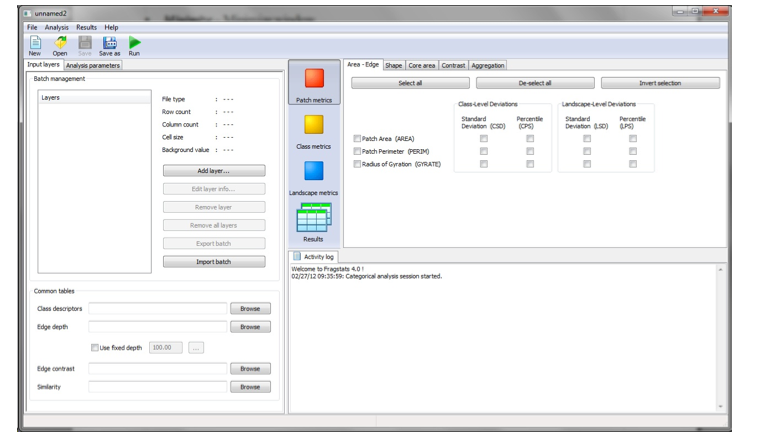
\includegraphics[width=\textwidth]{Introduccion/Figs/fragstatsmodeldialog}
\caption{Captura de pantalla del diálogo inicial de FRAGSTATS 4.0\label{fig:fragstatsmodeldialog}. Fuente: \url{www.landscapetoolbox.org}}
\end{figure}


Existen muchos otros programas especializados que permiten el cálculo de este tipo de métricas/índices pero no siempre tiene que ser una aplicación específica que las calcule. También es posible calcular facilmente determinadas métricas con \textbf{herramientas típicas de un SIG} de escritorio (calculadora de campos y/o calculadora raster, entre otras posibilidades).

En cualquier caso, no hay ninguna aplicación específica que sea escalable y extensible, y esté diseñada para realizar análisis sobre bases de datos de ocupación del suelo tan voluminosas y complejas como lo es la del SIOSE. Por ejemplo, según sus especificaciones técnicas, FRAGSTATS 4.0 es un software de 32 bits, lo cual significa que puede utilizar un máximo de 2GB de memoria, tampoco está diseñado para trabajar en \textit{La Nube} o con geometrías vectoriales.


\section{Objetivos}\label{sec:objetivos}

El principal objetivo de este trabajo es \textbf{desarrollar una extensión (PostgreSQL/PostGIS) que facilite el cálculo de métricas de paisaje}. Se quiere facilitar la realización de consultas y permitir el manejo de bases de datos voluminosas como lo es la base de datos \textit{actual} del SIOSE. 

Previsiblemente, las bases de datos de ocupación del suelo no harán sino aumentar en volumen y complejidad, por lo que si hoy en día existen los mencionados problemas de \textit{usabilidad} del SIOSE, estos no harán sino ir a más. De este modo el trabajo desarrollado tendrá continuidad en el tiempo.

Enlazando con el objetivo principal de este trabajo surgen objetivos más específicos relacionados con la metodología planteada en el proyecto SIOSE-INNOVA. En este sentido, se han considerado los siguientes \textbf{objetivos específicos}:
\begin{enumerate}
\item Aplicar herramientas de \textbf{desarrollo colaborativo} para trabajar con los otros investigadores del proyecto SIOSE-INNOVA.
\item Validar y testear la extensión desarrollada para comprobar su funcionamiento a partir de un \textbf{experimento con una geodatabase de usos del suelo de gran complejidad y volumen}, como es el SIOSE (2011).
\end{enumerate}

Es cierto que, a lo largo de este trabajo, se adquieren nuevos conocimientos sobre herramientas de desarrollo colaborativo, contenerización y orquestación, lenguajes de programación y lenguajes procedurales, además de aplicar prácticas y estándares de desarrollo más novedosos. Sin embargo, también se aplican todos los conocimientos adquiridos en el \textit{máster} de las distintas asignaturas impartidas sobre teoría e implementación de bases de datos, lenguajes de programación, software libre, aplicaciones infográficas y análisis espacial.


